\documentclass[12pt]{article}

% Packages
\usepackage[margin=1in]{geometry}
\usepackage{times}
\usepackage{graphicx}
\usepackage{booktabs}
\usepackage{amsmath}
\usepackage{amssymb}
\usepackage{float}
\usepackage{setspace}
\usepackage{natbib}
\usepackage{url}
\usepackage{indentfirst}
\usepackage{titlesec}
\usepackage{subcaption}
\usepackage{bbm}

% Set spacing and font size
\onehalfspacing
\renewcommand{\normalsize}{\fontsize{12pt}{14pt}\selectfont}
\setlength{\parindent}{0.5in}

% Format subsections (level 2 headings) - centered, italicized, not bold
\titleformat{\subsection}{\centering\normalsize\itshape}{}{0pt}{}

% Title and Author Information
\title{\normalsize The Impact of Employee Ownership Tax Credits on ESOP Plan Participation}
\author{\normalsize Mitchell Ballif, Patrick Beal, Will Cheney, and Soren Pack}
\date{}

\begin{document}

\maketitle

% Abstract
\begin{center}
\normalsize \textbf{ABSTRACT}
\end{center}

Write after analysis.

\vspace{12pt}

% Roman numeral counter for sections
\renewcommand{\thesection}{\Roman{section}}
\renewcommand{\thesubsection}{\Roman{subsection}}

% I. BACKGROUND
\section*{\centering \normalsize \textbf{I. BACKGROUND}}

\subsection*{A. Employee Stock Ownership Plans}

Employee Stock Ownership Plans (ESOPs) are retirement benefit plans that enable employees to acquire ownership stakes in their employer company. Instead of giving stock directly to individual employees, ESOPs function as trusts that hold company shares on behalf of plan participants. The trust maintains individual accounts for each participant, with allocations typically vesting over three to six years. When employees leave the company, employers must repurchase the shares of the employees, making sure the assets can be liquidated for employees who leave.

ESOPs are governed by the Internal Revenue Code and the Employee Retirement Income Security Act (ERISA), which require that these plans are broad-based and nondiscriminatory (29 U.S.C. \S 1107; 26 U.S.C. \S\S 4975, 409). Specifically, ESOPs must include all full-time employees who have worked at the company for at least a year, so that companies cannot use the plans to selectively reward individual employees. These regulations mean that once a company has established an ESOP, the whole workforce is included. Employees cannot opt out of being included in the plan, nor can they select into the plan except through their choice of where to work.

Two primary types of ESOPs exist: leveraged ESOPs and non-leveraged ESOPs. Leveraged ESOPs involve taking out loans with which the trust purchases company shares. The company then makes tax-deductible contributions to pay back the loan, with both principal and interest being deductible. Significant tax benefits come from this structure. Non-leveraged ESOPs involve direct contributions of company stock or cash to buy existing shares without borrowing loans. Both structures provide tax benefits to the ESOP plan sponsor, including deductible contributions, preferential treatment of S corporation ESOP shares at the federal level, and potential deductibility of dividends.

\subsection*{B. ESOP Data and Form 5500}

ERISA requires that all ESOP sponsors file Form 5500, which is the annual report of employee benefit plan information, with the U.S. Department of Labor, typically due by the end of July after the plan year. Form 5500 captures financial and operational data about the ESOP, including total assets, the number of plan participants, participant accounts, and contributions to the plan. For ESOPs specifically, Schedule E (ESOP Annual Information) must accompany the standard Form 5500 filing (see \citep{DOLForm5500ScheduleE}). ESOPs with 100 or more participants at the beginning of the plan year are required to attach audited financial statements to their Form 5500 filing. These public filings through the Department of Labor's EFAST2 system (\url{https://www.efast.dol.gov/}) create a comprehensive national dataset of ESOP participation and assets, making Form 5500 data a valuable empirical resource for studying the prevalence and impact of employee ownership structures at the firm level.

\subsection*{C. Colorado HB17-1214: Legislative Support for Employee Ownership Models}

In 2017, the Colorado legislature enacted House Bill 17-1214, signed by Governor John Hickenlooper, as a policy initiative to encourage transitions of existing small businesses to employee-owned models (Colorado General Assembly, HB17-1214, ``Encourage Employee Ownership Of Existing Small Business,'' \url{https://leg.colorado.gov/bills/hb17-1214}). The bill came as a recognition of a significant challenge in the employee ownership landscape, which is that while ESOPs and other employee ownership models provide significant benefits to workers and businesses, the costs and difficulty of switching to these models deters small businesses from transitioning (O'Boyle et al., 2016). The intent of this legislation was stated as reducing barriers to employee ownership conversion and establishing sustainable support mechanisms for Colorado businesses considering this transition.

The bill primarily focused on educational support and financing infrastructure rather than providing subsidies. It required the Colorado office of Economic Development and International Trade to contract with local nonprofit organizations that specialize in employee ownership to educate staff and promote employee ownership as part of the state's small business assistance services. The bill also set up a loan program to finance business transitions to employee-owned structures. It authorized annual appropriations of \$200,000 from the state general fund through 2022 to capitalize this loan program, with provisions allowing the state to accept additional private sector donations and to retain 15\% of loan repayments each year for administrative costs.

Businesses qualifying for the loan program were restricted to small businesses that were at least two years old with at least three employees, annual revenues below \$5 million, and a commitment to extend employee ownership opportunity to all workers. In 2019, after the initial implementation, Colorado expanded the program by setting up a grant program to help reduce costs more. Since this, Colorado has reportedly seen 20 to 25 businesses transition to employee ownership models each year. The original legislation intended for the program to end in July 2022, but the program has been extended, indicating the political support for the initiative.

% II. DATA
\section*{\centering \normalsize \textbf{II. DATA}}

We compile and merge data found on the U.S. Department of Labor website. Here they have publicly available pension plan information on all firms that have submitted a Form 5500. This data is split into two forms. Firstly, the long form which includes the plan information, including plan and company identifiers, plan type, and location of company. Secondly, each company must submit a Schedule H or a Schedule I depending on whether their plan has over or under 100 participants. The Schedule H and Schedule I datasets contain the same variables, the most important being the plan identification for linking and plan assets (both beginning of year and end of year). To obtain the dataset we used in the analysis, we first dropped all plans that are not pension plans, then merged the schedule I and H onto the long form. At this point, each observation was a unique pension plan. Therefore, to obtain the analysis we desired, we made two datasets. One we collapsed to the firm level so we can observe firm level outcomes. The second we collapsed to the state level so we could explore state level trends. The remainder of this data portion focuses mainly on these state level statistics as we are interested in treatment on the state level. To assess differences in ESOP characteristics across states, Table 1 displays summary statistics for Colorado, Utah, and the average of the other 48 states from 2011--2017.


\begin{table}[H]
\begin{center}
\caption{Summary statistics for Colorado, Utah, and other states (2011--2017)}
\label{fig:summary_stats}

\begin{tabular}{lrrrrrr}
\toprule
& \multicolumn{2}{c}{Colorado} & \multicolumn{2}{c}{Utah} & \multicolumn{2}{c}{USA} \\
\cmidrule(lr){2-3} \cmidrule(lr){4-5} \cmidrule(lr){6-7}
Variable & Mean & SD & Mean & SD & Mean & SD \\
\midrule
\addlinespace[0.5em]
Number of ESOP Firms & 117.83 & 5.98 & 56.83 & 2.14 & 129.62 & 142.02 \\
\addlinespace[0.5em]
Share of Firms with ESOP Plan & 0.04 & 0.00 & 0.04 & 0.00 & 0.05 & 0.02 \\
\addlinespace[0.5em]
ESOP Participants (BOY) & 33,930 & 778 & 26,228 & 906 & 279,316 & 362,909 \\
\addlinespace[0.5em]
ESOP Assets EOY (Millions USD) & 3,773 & 620 & 1,726 & 224 & 22,245 & 31,251 \\
\addlinespace[0.5em]
Active ESOP Participants (BOY) & 23,789 & 800 & 20,385 & 1,106 & 208,686 & 281,330 \\
\addlinespace[0.5em]
Total Active Pension Plan Participants & 880,878 & 30,849 & 495,848 & 28,830 & 1,553,037 & 1,738,323 \\
\addlinespace[0.5em]
Total Firms with Pension Plan & 2,938 & 168 & 1,591 & 64 & 3,169 & 3,727 \\
\addlinespace[0.5em]
\bottomrule
\end{tabular}

\vspace{0.5em}
{\small \textit{Notes: Means are computed over 2011--2017. The USA column represents the average across the remaining 48 states.}}

\end{center}
\end{table}


 In order to better visualize how trends over time differed in Utah and Colorado over the period of interest, Figures 1--4 compare Colorado and Utah across several key variables: Namely Active ESOP Participants (BOY), Total Firms with Pension Plan, ESOP Assets EOY (USD), and Number of ESOP Firms.

\begin{figure}[H]
\centering
\begin{minipage}{0.48\textwidth}
    \centering
    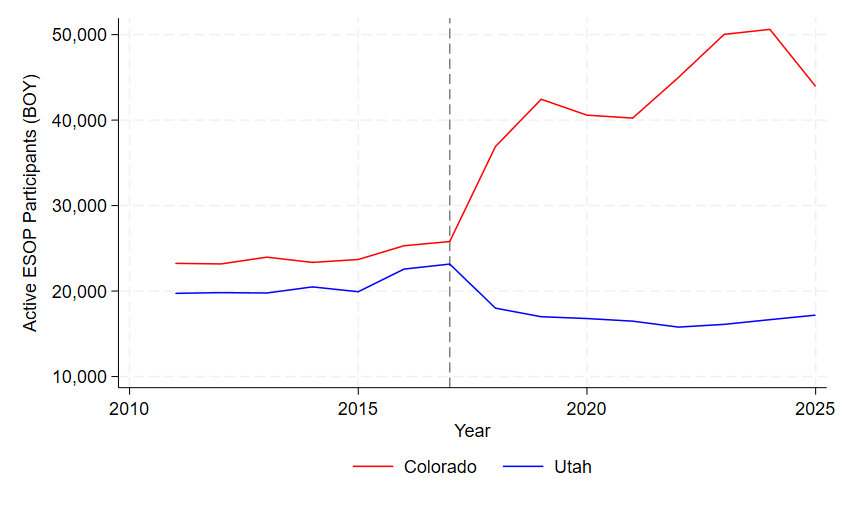
\includegraphics[width=\textwidth]{./images/data_portion/trend_comparison_tot_act_esop.png}
    \caption{Active ESOP Participants (BOY) - Colorado vs. Utah}
    \label{fig:active_participants_trend}
\end{minipage}
\hfill
\begin{minipage}{0.48\textwidth}
    \centering
    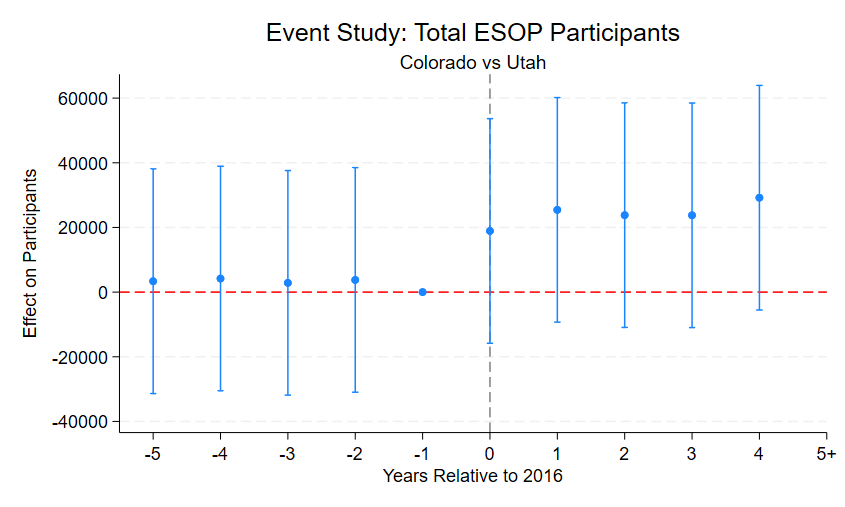
\includegraphics[width=\textwidth]{./images/data_portion/state_event_study_esop_participants.png}
    \caption{Active ESOP Participants (BOY) - Colorado vs. Utah}
    \label{fig:active_participants_event}
\end{minipage}
\end{figure}

\begin{figure}[H]
\centering
\begin{minipage}{0.48\textwidth}
    \centering
    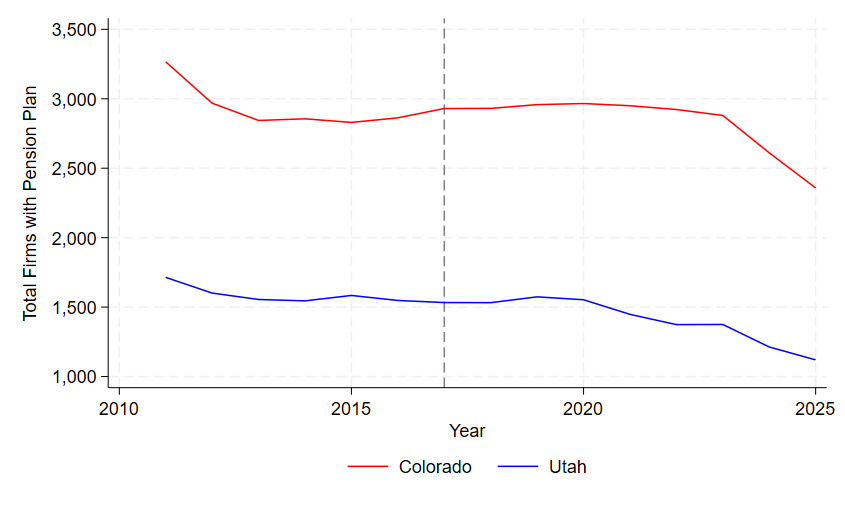
\includegraphics[width=\textwidth]{./images/data_portion/trend_comparison_total_firms.png}
    \caption{Total Firms with Pension Plan - Colorado vs. Utah}
    \label{fig:pension_firms_trend}
\end{minipage}
\hfill
\begin{minipage}{0.48\textwidth}
    \centering
    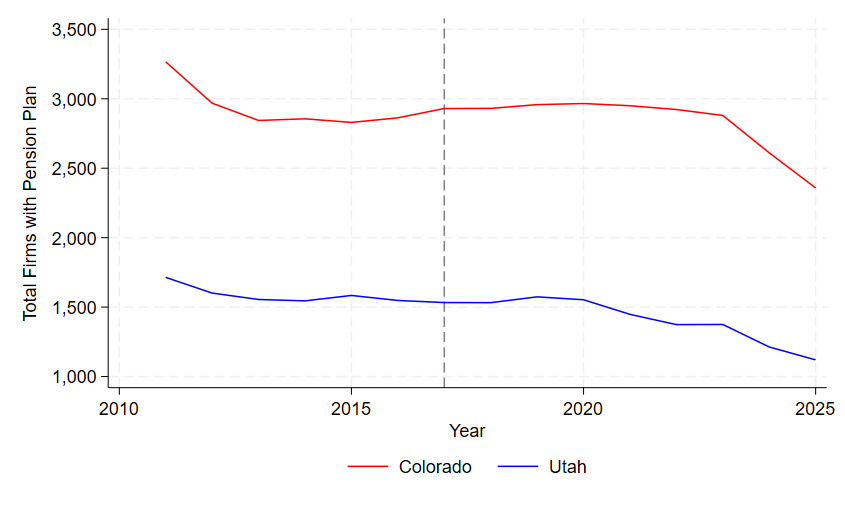
\includegraphics[width=\textwidth]{./images/data_portion/trend_comparison_total_firms.png}
    \caption{Total Firms with Pension Plan - Colorado vs. Utah}
    \label{fig:pension_firms_event}
\end{minipage}
\end{figure}

In Figures 1 and 3 we see similar trends in active ESOP participants and ESOP assets in Colorado and Utah across pre-treatment periods, with a sharp increase in Colorado in 2017 compared to Utah. This helps motivate our further analysis of the causal relationship between the legislation passed in 2017 and ESOP participation rates in the following sections. Interestingly, in Figures 2 and 4 the trends in total firms with a pension plan and number of ESOP firms for Utah and Colorado show little to no change in the years following 2017. We discuss the potential sources for these discrepancies between Figures 1 and 3 and Figures 2 and 4 in future sections where we further explore the causal relationship.

\begin{figure}[H]
\centering
\begin{minipage}{0.48\textwidth}
    \centering
    
\includegraphics[width=\textwidth]{./images/data_portion/trend_comparison_tot_esop_assets.png}
    \caption{ESOP Assets EOY - Colorado vs. Utah}
    \label{fig:esop_assets_trend}
\end{minipage}
\hfill
\begin{minipage}{0.48\textwidth}
    \centering
    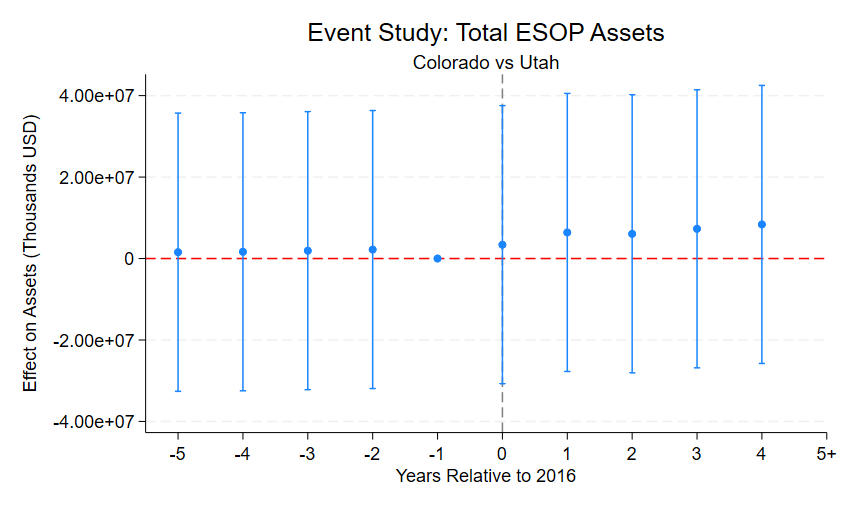
\includegraphics[width=\textwidth]{./images/data_portion/state_event_study_esop_assets.png}
    \caption{ESOP Assets EOY - Colorado vs. Utah}
    \label{fig:esop_assets_event}
\end{minipage}
\end{figure}

\begin{figure}[H]
\centering
\begin{minipage}{0.48\textwidth}
    \centering
    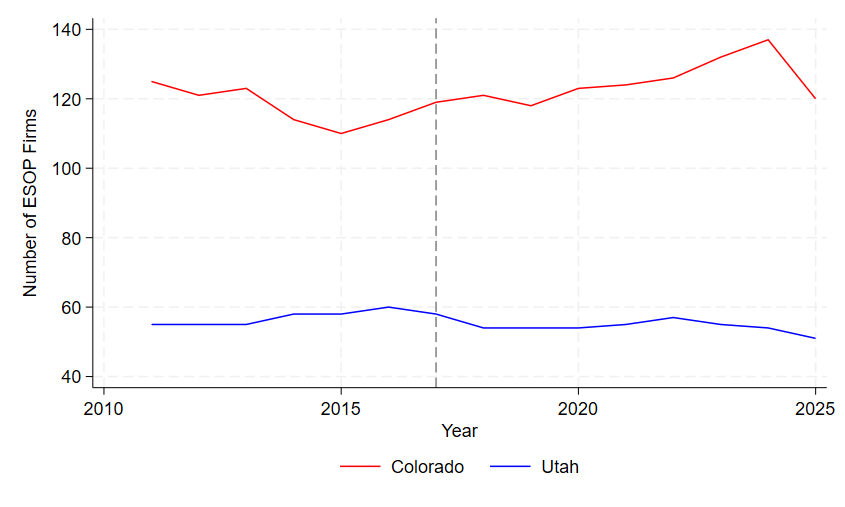
\includegraphics[width=\textwidth]{./images/data_portion/trend_comparison_num_esop_firms.png}
    \caption{Number of ESOP Firms - Colorado vs. Utah}
    \label{fig:esop_firms_trend}
\end{minipage}
\hfill
\begin{minipage}{0.48\textwidth}
    \centering
    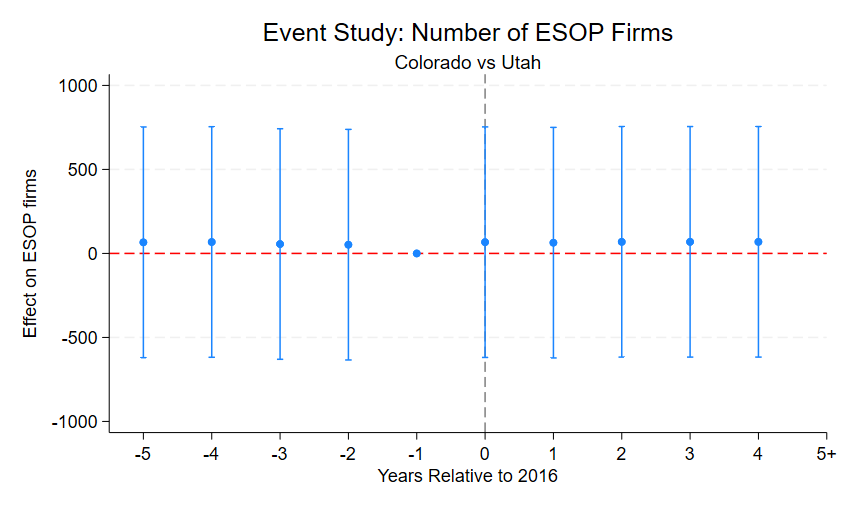
\includegraphics[width=\textwidth]{./images/data_portion/state_event_study_esop_firms.png}
    \caption{Number of ESOP Firms - Colorado vs. Utah}
    \label{fig:esop_firms_event}
\end{minipage}
\end{figure}

% III. METHODOLOGY
\section*{\centering \normalsize \textbf{III. METHODOLOGY}}

\subsection*{A. Estimation}

We employ a difference-in-differences (DiD) estimator to identify the causal effect of Colorado's HB17-1214 on ESOP participation. Our baseline specification is:

\begin{equation}
Y_{it} = \beta_0 + \beta_1 \text{DiD}_{it} + \gamma_s + \lambda_t + \epsilon_{it}
\end{equation}

where $Y_{it}$ represents one of the participation outcomes for firm $i$ in year $t$: an indicator for ESOP sponsorship, total ESOP plan participants, total ESOP assets (measure of participation intensity). The variable DiD$_{it}$ equals one if firm $i$ is in Colorado and year $t \geq 2017$. State fixed effects $\gamma_s$ control for time invariant differences between Colorado and Utah while year fixed effects $\lambda_t$ absorb common shocks. The coefficient $\beta_1$ identifies the average treatment effect under the parallel trends assumption.

Our primary regression compares Colorado (treatment) to Utah (control), selected for its geographic proximity, similar economic structure, and absence of competing employee ownership policies during our study period.

Due to identification concerns discussed later in the paper we verify robustness using synthetic control methods (Abadie, Diamond, and Hainmueller, 2010) with all U.S. states except Colorado as potential donors. For each outcome, we construct a synthetic Colorado as a weighted combination of control states that minimizes the mean squared prediction error over 2012--2016:


\begin{equation}
W^* = \arg\min_{W} \sum_{t=2012}^{2016} \left( Y_{Colorado,t} - \sum_{j \in \text{donors}} w_j Y_{j,t} \right)^2
\end{equation}

subject to $w_j \geq 0$ for all $j$ and $\sum_{j} w_j = 1$, where $W^* = (w_1^*, ..., w_J^*)$ are the optimal weights. The synthetic control uses pre-treatment ESOP rates in 2010, 2013, and 2016 as matching variables to ensure close alignment on outcome trends before the policy intervention in 2017.

\subsection*{B. Identification}

The validity of our DiD estimator rests on the parallel trends assumption: absent HB17-1214, ESOP participation in Colorado and Utah would have followed similar trajectories. While fundamentally untestable, we provide several pieces of evidence of common trends in the before treatment period in 2017.

We use an event study with the following specification to test our parallel trends assumption:

\begin{equation}
Y_{it} = \alpha + \sum_{\substack{k=-5 \\ k \neq -1}}^{5} \beta_k \mathbbm{1}[\text{Colorado}_i \times \text{Year}_{t}^k] + \gamma_i + \lambda_t + \epsilon_{it}
\end{equation}


where $k$ indexes years relative to treatment (2017), with $k=-1$ omitted as the reference period. The coefficients $\beta_k$ for $k < 0$ test for pre-existing differential trends between Colorado and Utah.

\begin{figure}[H]
\centering
\begin{subfigure}[b]{0.48\textwidth}
    \centering
    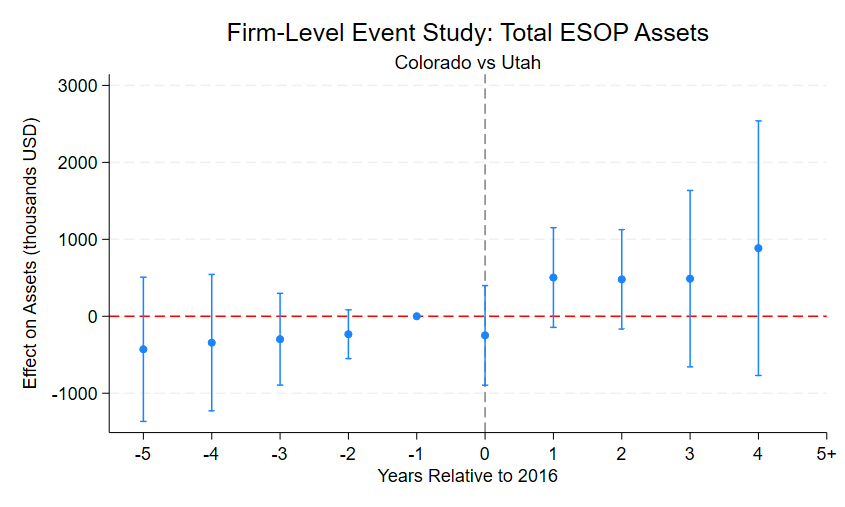
\includegraphics[width=\textwidth]{./images/data_portion/firm_event_assets.png}
    \caption{Specification 1}
    \label{fig:event_study_1}
\end{subfigure}
\hfill
\begin{subfigure}[b]{0.48\textwidth}
    \centering
    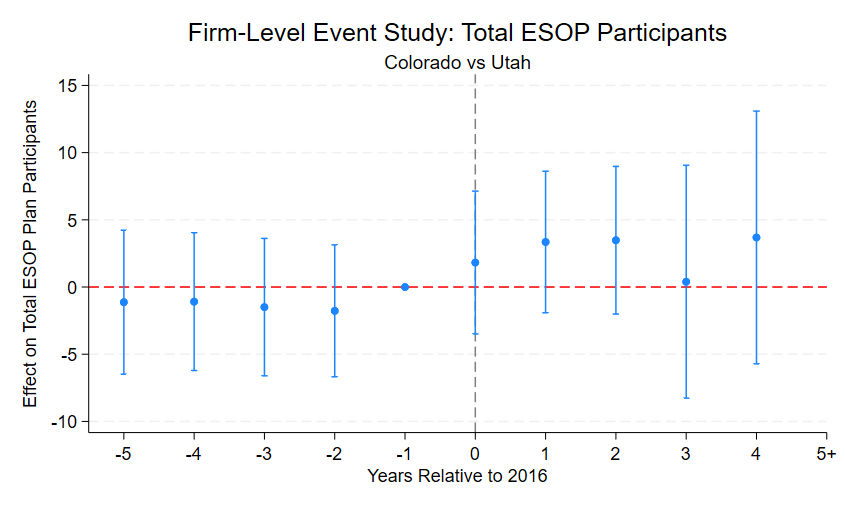
\includegraphics[width=\textwidth]{./images/data_portion/firm_event_partcp.png}
    \caption{Specification 2}
    \label{fig:event_study_2}
\end{subfigure}
\caption{Event Study Results}
\label{fig:event_study_both}
\end{figure}

The key identifying assumption is that no other shocks affected Colorado ESOP participation relative to Utah beginning in 2017 as demonstrated in event studies above. There is no statistically significant difference in effects on ESOP participation and assets before treatment in 2017. We view this as plausible given the states' similar economic conditions, but there are potential concerns when considering industry-specific differences. Our state fixed effects control for time-invariant factors, but cannot rule out industry-specific shocks coinciding with treatment. For example, if Colorado's professional services sector experienced particularly strong growth after 2017 while Utah's manufacturing sector faced different trends, this could differentially affect ESOP adoption patterns independently of the Colorado Bill. Similarly, state-specific changes in tax policy or retirement plan legislation could confound our estimates if they coincided with the policy rollout. Our research failed to identify any such shock.

Potential violations of SUTVA through spillovers to Utah through firm cross-border firm employee behavior while possible appear to be very unlikely due to the nature of small business employee ownership transitions. Moreover, Form 5500 classifies firms based on their headquarters location, meaning that spillovers would only bias our estimates if they induced Utah-headquartered firms to adopt ESOPs. Firms with Colorado operations but Utah headquarters would be classified as Utah firms in our data, further limiting potential spillover concerns.

\subsection*{C. Issues and Robustness}

Several challenges question the validity of our estimates, though we argue these do not fundamentally undermine our central finding: Colorado's HB17-1214 had at most modest, and likely negligible, effects on ESOP participation.

\textit{Clustering and Inference:} A fundamental challenge in our design is that treatment is assigned at the state level while our outcomes are measured at the firm level. The theoretically appropriate procedure would cluster standard errors at the state level to account for correlated shocks within states over time, however with only two states, state-level clustering is infeasible. We therefore cluster at the firm level, which accounts for serial correlation within firms but substantially understates standard errors relative to the appropriate state-level clustering. This creates a severe inference problem: our reported standard errors and p-values are likely misleading, potentially overstating the precision of our estimates. While our point estimates remain unbiased under standard DiD assumptions, we cannot reliably conduct hypothesis tests or construct confidence intervals. Interestingly enough, this works in favor of our null findings: if state-level clustering were feasible, our standard errors would be dramatically larger, making our already-insignificant results even more clearly insignificant.

\textit{Sample Size:} Our analysis compares a single treatment state (Colorado) to a single control state (Utah), providing minimal variation to identify treatment effects. This severely limits our ability to distinguish treatment effects from Colorado-specific shocks occurring after 2017. While we observe many firms within each state, the effective sample size for identifying the treatment effect is essentially two states. This constraint makes our estimates especially vulnerable to bias from any Colorado-Utah differences in post-2017 trends unrelated to HB17-1214.

\textit{Confounding Variables:} Firm participation in pension plans is highly dependent on profitability, employee turnover, competing benefit offerings, regulatory costs, and management preferences. These factors may vary systematically across states due to labor market conditions, industry composition, or unrelated state policies. If Colorado experienced differing trends in 401(k) adoption for example after 2017, these could mask true ESOP effects or generate spurious correlations. Our fixed effects control for time-invariant differences and common trends but cannot account for state-specific time-varying factors. Given the complex determinants of pension plan participation, small treatment effects could easily be masked by other factors influencing firms' benefit decisions.

While evidence supports unbiased estimates through pre-treatment parallel trends, the consistency of our standard errors remains severely limited. With only two states, we cannot construct consistent variance estimates. Our synthetic control analysis partially addresses these concerns by constructing a counterfactual using all U.S. states as donors, which reduces dependence on Utah as the sole control and provides some evidence of more substantial effects for certain outcomes. However, fundamental challenges remain. To more definitively bolster inference, we suggest multi-state designs using proper state-level clustering through: (1) a TWFE design exploiting staggered adoption of employee ownership policies across multiple states, or (2) accessing private ownership data to conduct regression discontinuity around the 30\% ESOP ownership threshold that triggers specific tax advantages. Despite these limitations, the overall pattern of small to modest effects across our firm-level and synthetic control specifications suggests minimal policy impact.

% IV. RESULTS
\section*{\centering \normalsize \textbf{IV. RESULTS}}

\subsection*{A. Main Results: Outcome Variables}

We estimate a two-way fixed effects difference-in-differences specification comparing Colorado (treated state) and Utah (control state). The outcome variables are:

\begin{itemize}
\item (1) ESOP Firm: Indicator for ESOP presence
\item (2) Total Participants: esop\_tot\_partcp\_by\_cnt
\item (3) Total Assets: esop\_tot\_assets\_by\_amt (in dollars)
\item (4) Active Participants: esop\_tot\_active\_partcp\_cnt
\item (5) Participation Rate: esop\_partcp\_rate
\end{itemize}

\subsubsection*{Model 1: Year and State Fixed Effects}

\textbf{Specification:}

\texttt{reghdfe outcome did if state\_fips == 8 | state\_fips == 49, \\ absorb(state\_fips year) vce(cluster spons\_dfe\_ein)}
\begin{table}[H]
\centering
\caption{Difference-in-Differences Results: Year and State Fixed Effects}
\label{tab:model1}
\footnotesize

\begin{tabular}{lccccc}
\toprule
Variable & (1) ESOP Firm & (2) Total Partcps. & (3) Total Assets & (4) Active Partcps. & (5) Partcp. Rate \\
\midrule
\textbf{DID} & 0.00607 & 25.19 & 2,878,102.7* & 22.29 & 0.00613 \\
             & (0.00486) & (17.35) & (1,611,044.2) & (15.37) & (0.00426) \\
\textbf{Constant} & 0.0215*** & 18.16*** & 1,258,818.5*** & 13.99*** & 0.0175*** \\
                  & (0.00131) & (6.636) & (445,403.5) & (5.124) & (0.00113) \\
\midrule
\textbf{Observations} & 209,399 & 209,399 & 209,399 & 209,399 & 191,912 \\
\bottomrule
\end{tabular}

\vspace{0.5em}
{\footnotesize Standard errors in parentheses; * $p<0.10$, ** $p<0.05$, *** $p<0.01$}
\end{table}


\textbf{Interpretation:} The only statistically significant result is total ESOP assets, significant at the 10\% level. However, an increase of approximately \$2.9 million in assets is likely not economically significant relative to Colorado's total ESOP holdings. The ESOP firm indicator shows a small, insignificant increase of 0.006 percentage points. The participation rate results are comparable to the firm indicator, suggesting minimal policy impact on worker participation. Total participants (25.19) and active participants (22.29) are not statistically significant. Given Colorado's population and economy, these small changes lack economic significance.

A key methodological note: we cluster standard errors at the firm level despite state-level treatment assignment because comparing only two states makes state-level clustering infeasible. Firm-level clustering accounts for within-firm correlation over time.

\subsubsection*{Model 2: Year Fixed Effects Only}

\textbf{Specification:}

\texttt{reghdfe outcome did treat if state\_fips == 8 | state\_fips == 49, \\ absorb(year) vce(cluster spons\_dfe\_ein)}

\begin{table}[H]
\centering
\caption{Difference-in-Differences Results: Year Fixed Effects Only}
\label{tab:model2}
\footnotesize
\begin{tabular}{lcccc|c}
\toprule
Variable & (1) ESOP Firm & (2) Total Partcps. & (3) Total Assets & (4) Active Partcps. & (5) Partcp. Rate \\
\midrule
\textbf{DID} & 0.00607 & 25.19 & 2,878,102.7* & 22.29 & 0.00613 \\
 & (0.00486) & (17.35) & (1,611,044.2) & (15.37) & (0.00426) \\
\textbf{Treat} & -0.00100 & -21.17 & -1,344,888.2 & -20.00 & 0.0000977 \\
 & (0.00213) & (15.07) & (1,027,215.5) & (14.25) & (0.00182) \\
\textbf{Constant} & 0.0222*** & 32.36*** & 2,160,957.6*** & 27.40*** & 0.0174*** \\
 & (0.00206) & (9.960) & (709,935.7) & (10.21) & (0.00174) \\
\midrule
\textbf{Observations} & 209,399 & 209,399 & 209,399 & 209,399 & 191,912 \\
\bottomrule
\end{tabular}

\vspace{0.5em}
{\footnotesize Standard errors in parentheses; * $p<0.10$, ** $p<0.05$, *** $p<0.01$}
\end{table}

\subsubsection*{Model 3: State Fixed Effects Only}

\textbf{Specification:}

\texttt{reghdfe outcome did post if state\_fips == 8 | state\_fips == 49, \\ absorb(state\_fips) vce(cluster spons\_dfe\_ein)}

\begin{table}[H]
\centering
\caption{Difference-in-Differences Results: State Fixed Effects Only}
\label{tab:model3}
\footnotesize
\begin{tabular}{lcccc|c}
\toprule
Variable & (1) ESOP Firm & (2) Total Partcps. & (3) Total Assets & (4) Active Partcps. & (5) Partcp. Rate \\
\midrule
\textbf{DID} & 0.00671 & 25.59 & 2,941,710.8* & 22.47 & 0.00669 \\
 & (0.00486) & (17.29) & (1,620,237.0) & (15.18) & (0.00426) \\
\textbf{Post} & 0.0199*** & -18.67 & -778,399.0 & -18.47 & 0.0158*** \\
 & (0.00384) & (13.86) & (1,146,090.0) & (13.17) & (0.00329) \\
\textbf{Constant} & 0.0178*** & 21.52*** & 1,393,177.1*** & 17.33*** & 0.0144*** \\
 & (0.000998) & (7.304) & (485,252.2) & (6.140) & (0.000857) \\
\midrule
\textbf{Observations} & 209,402 & 209,402 & 209,402 & 209,402 & 191,915 \\
\bottomrule
\end{tabular}

\vspace{0.5em}
{\footnotesize Standard errors in parentheses; * $p<0.10$, ** $p<0.05$, *** $p<0.01$}
\end{table}

\textbf{Robustness Check:} Removing year or state fixed effects yields highly similar coefficient estimates and significance levels. The DID coefficient remains stable across specifications, indicating results are robust to the choice of fixed effects structure.

\subsubsection*{Synthetic Controls}

\begin{figure}[H]
\centering
\includegraphics[width=0.7\textwidth]{./images/image8.png}
\caption{Synthetic Control Results - Outcome 1}
\label{fig:synth_control_1}
\end{figure}

\begin{figure}[H]
\centering
\includegraphics[width=0.7\textwidth]{./images/image9.png}
\caption{Synthetic Control Results - Outcome 2}
\label{fig:synth_control_2}
\end{figure}

\begin{figure}[H]
\centering
\includegraphics[width=0.7\textwidth]{./images/image10.png}
\caption{Synthetic Control Results - Outcome 3}
\label{fig:synth_control_3}
\end{figure}

\begin{figure}[H]
\centering
\includegraphics[width=0.7\textwidth]{./images/image11.png}
\caption{Synthetic Control Results - Outcome 4}
\label{fig:synth_control_4}
\end{figure}

\begin{figure}[H]
\centering
\includegraphics[width=0.7\textwidth]{./images/image12.png}
\caption{Synthetic Control Results - Outcome 5}
\label{fig:synth_control_5}
\end{figure}

Using Synthetic Controls as a way to check robustness we can see that the effects are more significant. These synthetic controls were done on all of the states and not just Colorado and Utah. The synthetic controls were made from various states. In these synthetic controls the pre-trends match very closely. After the treatment occurs, it appears Colorado has a larger growth than the synthetic control. This implies that the legislation passed in had some effect on the amount of ESOP firms and participation within those firms. This differs from what we found in the Difference in Difference between Utah and Colorado where we found little significance. This implies that more research needs to be done on this.

% V. CONCLUSION
\section*{\centering \normalsize \textbf{V. CONCLUSION}}

\vspace{12pt}

Despite clear pre-treatment parallel trends between Colorado and Utah, our analysis finds limited evidence that Colorado's HB17-1214 substantially increased ESOP participation at the firm level. Our two-way fixed effects estimates show small, mostly insignificant effects across key outcomes. Only total ESOP assets shows marginal significance $(p < 0.10)$ with an increase of approximately \$2.9 million, an economically modest change relative to Colorado's total ESOP holdings. Point estimates for ESOP firm presence, total participants, and participation rates are all small and statistically indistinguishable from zero.

These findings face important methodological constraints. Most critically, with treatment assigned at the state level but outcomes measured at the firm level, proper inference requires state-level clustering. However, comparing only two states makes this infeasible. Our firm-level clustered standard errors substantially understate uncertainty, meaning even our one marginally significant result should be interpreted cautiously. Moreover, our design cannot definitively rule out Colorado-specific trends after 2017 unrelated to HB17-1214. Changes in industry composition, competing state policies, or labor market conditions could mask true effects or generate spurious correlations.

Our synthetic control analysis using all U.S. states as potential donors suggests somewhat larger effects, particularly for ESOP participation and assets, where Colorado appears to outperform its synthetic counterfactual after 2017. However, synthetic controls face their own severe identification challenges. The method assumes that the weighted combination of control states provides a valid counterfactual for Colorado absent treatment. This assumption becomes questionable if unobserved state-specific shocks after 2017 differentially affected states with different weights in the synthetic control. The apparent divergence between our difference-in-differences and synthetic control results highlights rather than resolves the fundamental identification problem: with a single treated state and limited pre-treatment periods, we cannot confidently distinguish policy effects from coincidental state-specific trends.

The most straightforward interpretation is that Colorado's legislation had minimal impact on ESOP adoption and participation during our study period. This does not necessarily imply the policy failed. The program emphasized education and financing infrastructure rather than direct subsidies, and such foundational investments may require longer timeframes to influence firm behavior than our 2012-2019 window captures. Additionally, if the policy primarily affected firm survival or intensive-margin changes within existing ESOPs rather than extensive-margin adoption, our specifications may not detect these effects.

Future research should exploit staggered adoption of employee ownership policies across multiple states to enable proper state-level inference. A multi-state differences-in-differences design would provide the statistical power our two-state comparison lacks. Our analysis demonstrates both the promise of Form 5500 data for studying employee ownership and the challenges of evaluating state-level policies with limited cross-sectional variation.

% References
\section*{\centering \normalsize \textbf{VI. REFERENCES}}
% Prevent the bibliography environment from printing its own heading (avoid double 'References')
\renewcommand{\bibsection}{}
\bibliographystyle{apalike}
\nocite{*}
\bibliography{references}

\end{document}
